\documentclass{article}
\usepackage[utf8]{inputenc}

\title{Proposta de priorização de áreas de restauração na Bacia Hidrográfica do Rio Doce: Como usar os resultados de Strassburg et al. 2019?}
\author{Grupo NCCG-JBRJ}
\date{March 2020}

\usepackage{biblatex}
% Eu vi que o Overleaf tem a opção de conectar o .bib com o Mendeley, mas é só na versão paga. Acho que vamos ter que ir atualizando o .bib manualmente, quando necessário
\addbibresource{refs_proj2PCI_20-03-2020.bib}
\usepackage{graphicx}

\begin{document}

\maketitle

\section{Breve descrição do estudo}
O estudo de Strassburg et al. \cite{Strassburg2019} investigou cenários alternativos para a restauração ecológica na Mata Atlântica. Os autores utilizaram a abordagem de priorização baseada em programação linear. A priorização foi baseada em três cenários básicos (Figura \ref{fig:results}): 

\begin{itemize}
    \item Biodiversidade: Diminuição do risco  de extinção associado ao aumento de áreas de habitat adequados para cada espécie
    \item Mudanças climáticas: Aumento do sequestro de carbono em áreas degradadas
    \item Custos: Valor gasto em restauração, incluindo o potencial de perda de receita da agricultura ou pecuária de áreas que estão sendo restauradas
\end{itemize}
 
Além dos três anteriores, foi proposto um cenário "final", combinando o melhor possível dos três objetivos: maximização da biodiversidade, maximização de sequestro de carbono e diminuição de custos (Figura \ref{fig:results}).

\section{Como poderia ser aplicado no nosso primeiro produto}
Inicialmente foi feito um recorte simples do cenário final de Strassburg et al. \cite{Strassburg2019} para a área da Bacia Hidrográfica do Rio Doce (BHRD, Figura \ref{fig:scenarios_BHRD}).

No entanto, este simples recorte gera um erro de interpretação nos valores dos pixels, por causa da diferença de escala. No resultado original de Strassburg et al. \cite{Strassburg2019}, os valores representam quantas vezes o pixel foi considerado prioritário em relação aos demais pixels da área de estudo (toda a Mata Atlântica). Portanto, esta "prioridade relativa" não faz sentido somente para a área da BHRD.
%ast. nao sei se para o texto, mas para analisar, a gente precisa relembrar as camadas que foram usadas nessa priorizacao do iis. camada biotica ok, endemicas com mais de 10 registros, modeladas com 3 algoritmos. o resto foi custo de orpotunidade mesmo e mais o que? 
Sugestão: Descrever as características particulares da BHRD relevantes para a tomada de decisão em restauração (biodiversidade, uso do solo incluindo mineração, áreas protegidas) e, posteriormente, discutir/comparar com a análise em macroescala, na Mata Atlântica, feita por Strassburg et al. \cite{Strassburg2019}.

\section{Proposta para o primeiro produto}

Perguntas para guiar a execução do primeiro produto (divisão preliminar de tarefas):

\begin{itemize}
    \item Biodiversidade:
    \begin{enumerate}
        \item Quais são as espécies vegetais de ocorrência na BHRD? 
        \item Quais delas são endêmicas? Quais têm distribuição restrita (baseando-se no critério da IUCN, por exemplo)?
        \item Como as espécies são distribuídas nas microbacias? 
        \item Quais são as áreas de maior riqueza na BHRD?
    \end{enumerate}
    
    \item Uso do solo:
    \begin{enumerate}
        \item Como se distribuem as diferentes classes de uso do solo na BHRD? 
        \item Essa distribuição é uniforme ao longo da BHRD ou varia nas diferentes microbacias? Como varia?
        \item Quais microbacias possuem maior cobertura vegetal?
        \item Qual é a proporcão da área ocupada por cada uma delas na bacia?
        \item ...
    \end{enumerate}
    
    \item Mineração:
    \begin{enumerate}
        \item Qual é a porcentagem da área total da BHRD usada para mineração?
        \item Quantas destas áreas estão em atividade? Quantas estão planejadas?
        \item Como a área destinada a mineração na BHRD mudaria com as PLs propostas: PL 37/2011 (propõe permitir mineração em UCs de uso sustentável), PL 3682/2012 (permite mineração em até 10\% da área de UCs de proteção integral) e PL 1610/1996 (permite mineração em terras indígenas).
    \end{enumerate}
    
    \item Áreas protegidas:
    \begin{enumerate}
        \item Qual é a porcentagem da área total da BHRD já protegida por UCs?
        \item Qual o tamanho das UCs? São fragmentos grandes ou pequenos e como estes fragmentos (UCs) estão conectados entre si?
        \item Como é a distribuição de UCs nas diferentes microbacias? 
        \item Como é o entorno dessas UCs?
    \end{enumerate} 

    \item Áreas para restauração:
    \begin{enumerate}
        \item Baseando-se nas respostas das perguntas anteriores, conseguimos apontar áreas "receptíveis" à restauração? Não sei se faz sentido, mas seria uma primeira avaliação, antes da priorização, que dependerá dos modelos das espécies (segundo produto?).
        \item 
    \end{enumerate} 
\end{itemize}


\begin{figure}[h!]
\centering
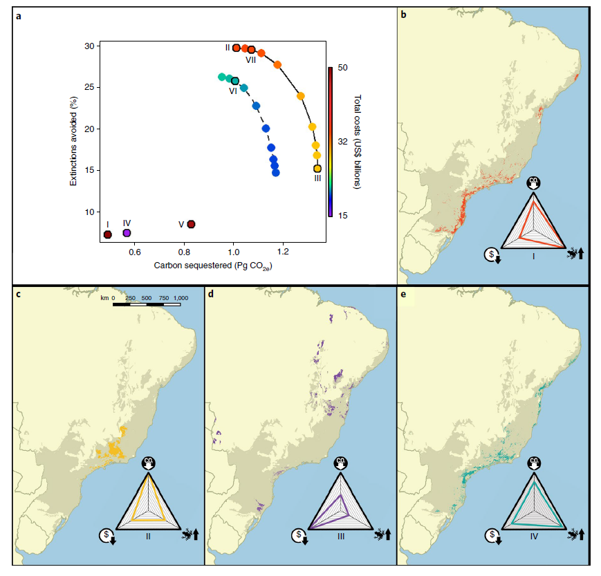
\includegraphics[scale=0.6]{figs/main_results.png}
\caption{Cenários de restauração ecológica na Mata Atlântica \cite{Strassburg2019}}
\label{fig:results}
\end{figure}

\begin{figure}
    \centering
    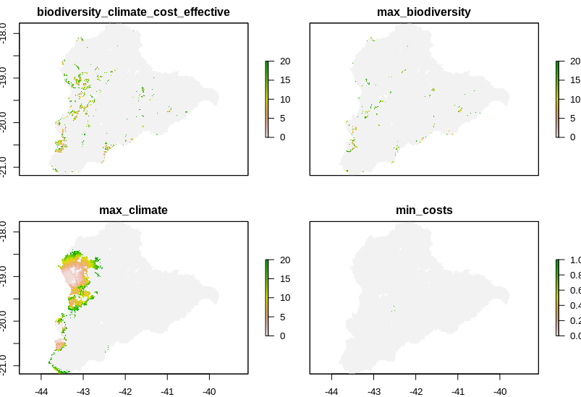
\includegraphics[scale=0.7]{figs/scenarios_BHRD.png}
    \caption{Cenários de Strassburg et al. \cite{Strassburg2019} cortados para a área da Bacia Hidrográfica do Rio Doce}
    \label{fig:scenarios_BHRD}
\end{figure}

\section{Requisitos e alternativas para uma priorização no âmbito do PCI}%ast srm
Um cenário de priorização da conservação ou da restauração na escala da Bacia vai precisar dos seguintes elementos: 

\begin{itemize}
    \item A definição do objetivo da priorização: conservação ou restauração? e levando em conta quais premissas? O planejamento estratégico para conservação foi desenhado inicialmente no contexto da conservação e adaptações posteriores são as que têm falado de restauração (inclusive Strassburg) %ast isso também sou eu pegando o bonde andando, acho.
    \item O levantamento e a definição dos dados que serão utilizados. Basicamente camada(s) biótica(s) e camadas de variáveis abióticas -mas quais e como - a lista elencada na proposta está boa, mas é preciso detectar se falta alguma variável essencial para responder a pergunta ou se sobra alguma. Algumas destas variáveis que faltam não são nada triviais de se obter e podem requerir que a gente faça uma parceria p.ex. com o IIS, seja com eles facilitando código e cálculos que lhes permitem gerar essas camadas (econômicas, estoque de carbono, custo de oportunidade), ou idealmente gerando essas camadas, com a extensão e resolução que o projeto definir. %A gente acha (srm, ast) que esta fase é a única que pode ser de fato implementada em um curto período de tempo mas elencar isto bem é crucial para qualquer produto futuro. 
    \item A escolha do método mais apropriado para a priorização. Fora softwares comerciais clássicos (zonation, marxan) e scripts privados %uma pena que não sejam disponibilizados
    tem o pacote prioritizr de R que usa uma licença comercial para a optimização. 
    
\end{itemize}

\printbibliography
\end{document}
